
\subsection*{Mise en situation}

En escalade, en l’absence de points de liaison permanents (pitons, broches scellés…), l’assurage peut être complété par des coinceurs, qui se placent dans les fissures, et se bloquent sous le choc en cas de chute. C’est l’adhérence qui permet la retenue de la chute.
\begin{center}
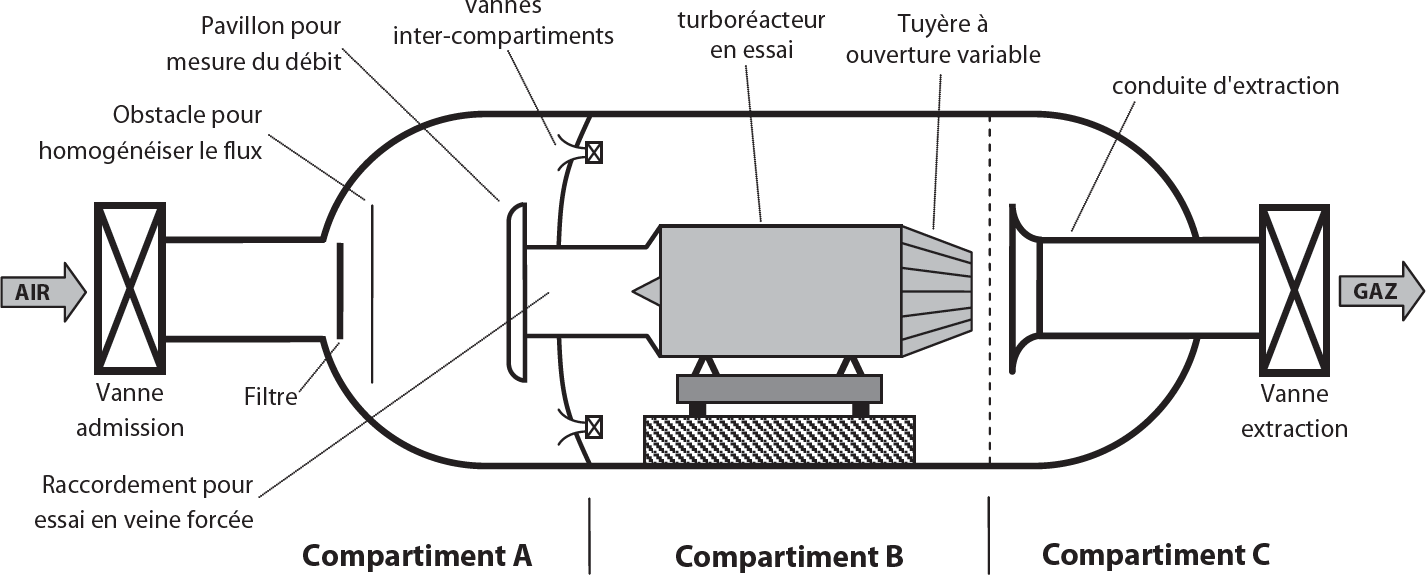
\includegraphics[height = 3cm]{fig_02}
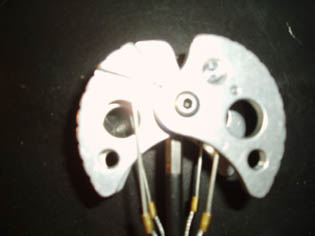
\includegraphics[height = 3cm]{fig_03}
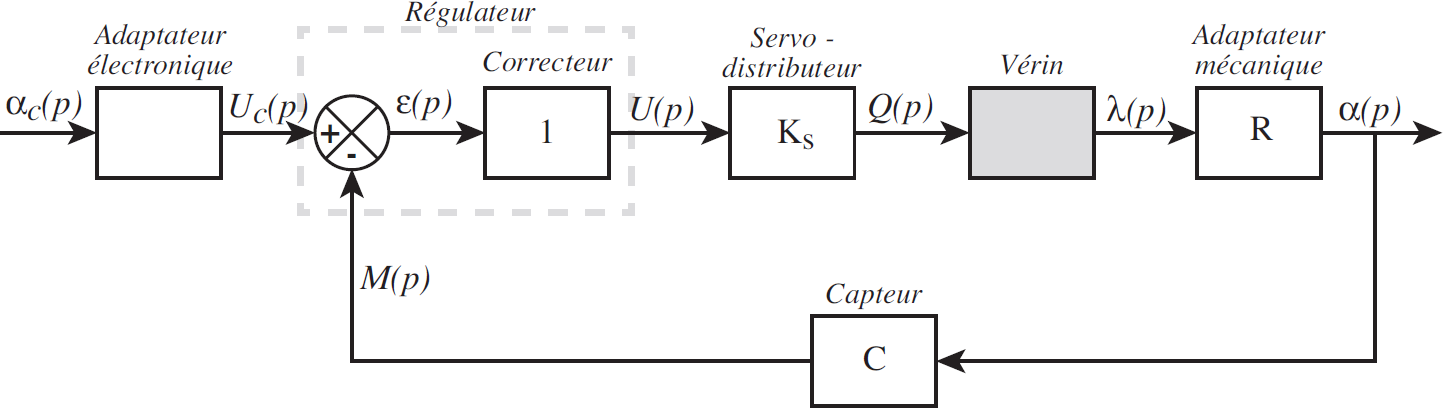
\includegraphics[height = 3cm]{fig_04}
\end{center}
Il existe des coinceurs monoblocs, qui permettent un coincement dans une fissure à bords convergents, mais les 
«~friends~» à came, articulés sont très supérieurs en cela qu’ils permettent une protection dans des fissures à bords parallèles. De plus, leur géométrie leur permet de s’adapter à des fissures de tailles différentes (par exemple de 55 à \SI{90}{mm} pour un «~flex no~4 »).

On se propose d’étudier les conditions de retenue d’un coinceur « Rock Empire Flex » schématisé ci dessous, en modélisation plane. Dans le cadre de ce modèle, on considère donc les 2 camas, l'axe cylindrique et les parois supposées parallèles. 


\begin{center}
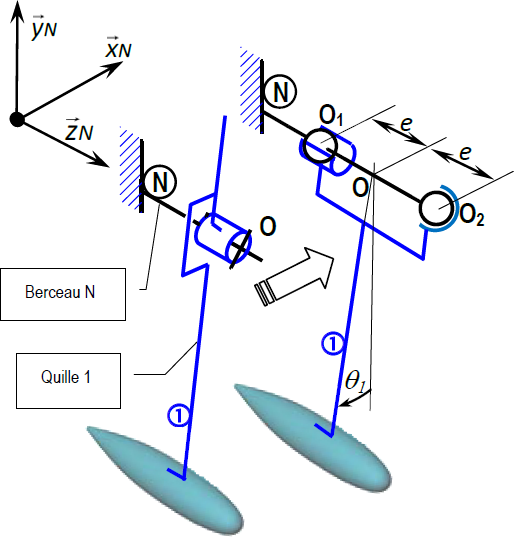
\includegraphics[width=\linewidth]{fig_05}
\end{center}

\question{Réaliser un graphe de liaisons.}
\ifprof
\begin{corrige}~\\
\end{corrige}
\else
\fi


\question{Sur la figure précédente, indiquer la direction et le sens des efforts normaux et tangentiels.}
\ifprof
\begin{corrige}~\\
\end{corrige}
\else
\fi

\question{Déterminer le coefficient de frottment permettant d'encaisser l'effort de la chute.}
\ifprof
\begin{corrige}~\\
\end{corrige}
\else
\fi

\question{Quel est l’effort d’écartement imposé aux lèvres de la fissure sous 10 000 daN de traction (composante normale à la surface du rocher) ?}
\ifprof
\begin{corrige}~\\
\end{corrige}
\else
\fi

\question{Sur le corps du coinceur, il est porté : \textbf{Maxi : \SI{12}{kN}}. Y a-t-il  risque de glissement au delà de cette charge ? pourquoi ? et que se passe-t-il alors ?}
\ifprof
\begin{corrige}~\\
\end{corrige}
\else
\fi

\subsection*{Pour aller plus loin : profil idéal de la came}

Nous allons, dans cette partie, rechercher le profil idéal de la came du coinceur, en supposant
que le coefficient de frottement minimal obtenu précédemment est valide pour toutes les largeurs
de fissure.

On se place dans le cas de la fissure la plus large (contact en $A$ avec le rocher). Soient $r_0$ la
distance $OA$, $L_{f0}$ la largeur totale de la fissure, $f_0 = \tan \varphi_0$ le coefficient de frottement coinceur / roche minimal déterminé précédemment (qui pourrait être déterminé expérimentalement dans
le cadre de la conception du coinceur).

\question{En appliquant judicieusement le principe fondamental de la statique, établir la relation entre
$r_0$, $L_{f0}$ et $\varphi_0$. On remarque que pour l’instant, on n’étudie qu’une seule largeur de fissure, le
raisonnement pouvant être étendu à d’autres.}

Afin que le contact rocher / came du coinceur se fasse au bon endroit, dans le cas d’une fissure
à bords parallèle, il faut s’assurer que la tangente à la courbe de la came au niveau du point de
contact $B$ soit dirigée suivant $\vect{y}$ (voir figure ci-dessous). Le profil de la came peut être exprimé
sous la forme d’une équation polaire $r(\theta) = f(\theta)$ avec $f$ une fonction à déterminer. On considère
que $\theta=0$ pour la plus grande largeur de fissure $L_{f0}$ (associée au contact au point $A$).

\begin{center}
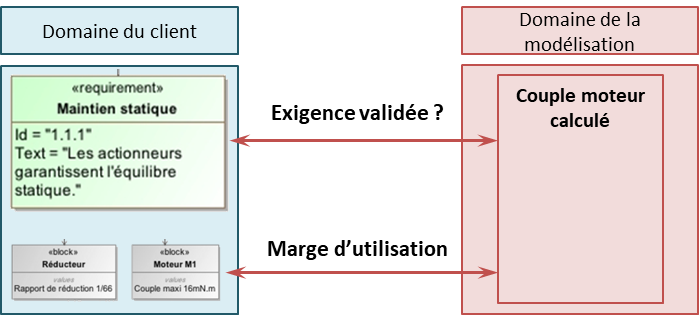
\includegraphics[width=\linewidth]{fig_06}
\end{center}


\question{L’angle $\dd \theta$ étant faible, on peut considérer que le triangle $IJB$ est rectangle en $I$. Déterminer à partir de relations géométriques dans ce triangle la relation entre $\dfrac{\dd r}{\dd \theta}$, $r(\theta)$ et $\varphi_0$.
Mettre l’équation obtenue sous la forme d’une équation différentielle du premier ordre.}

\question{Résoudre l’équation différentielle précédente en considérant que pour $\theta = 0$ (contact en $A$),
$r(\theta = 0) = r_0$, avec $r_0$ le rayon déterminé précédemment en fonction de $L_{f0}$. Tracer l’allure
du profil de came obtenu, en considérant que le coinceur doit s’adapter à des largeurs de
fissures allant de 65 à \SI{90}{mm} (caractéristiques du coinceur flex n 4), et que $\varphi_0 = 9\degres = \SI{0,157}{rad}$. La forme de came calculée vous semble-t-elle correspondre à la forme réellement
utilisée par le constructeur ?}